
"Finally, by making different things intended to address the same problematic situation, RtD can reveal design patterns \autocite{Alexander_book} around problem framings, around specific interactions, and around how theory can be operationalized" \autocite[p. 178]{zimmerman_research_2014}.


The initial problem framing was concerned with designing an installation that addresses sustainability, which triggered a design process and conceptual exploration of sustainability-themes worthy of investigation. Guided by this framing I chose to explore \emph{the relationship between human and nature}. Through literature review (Chapter 2), essay-writings (see appendix) and prototyping (see Chapter 8: Exploring input through plants) I learned that elements, or qualities,


Main RQ: How can one design meaningful interactive experiences in a museum space that addresses sustainability?
answered by: objectifying meaningfulness as a quality that you can design for in a museum.
through: finding/identifying dialogic relations between visitor and installation.


The main purpose of this analysis-oriented part is to contribute with knowledge that make visible dialogic qualities between interactive installations and visitor-experience. 



\begin{figure}[H]
\centering
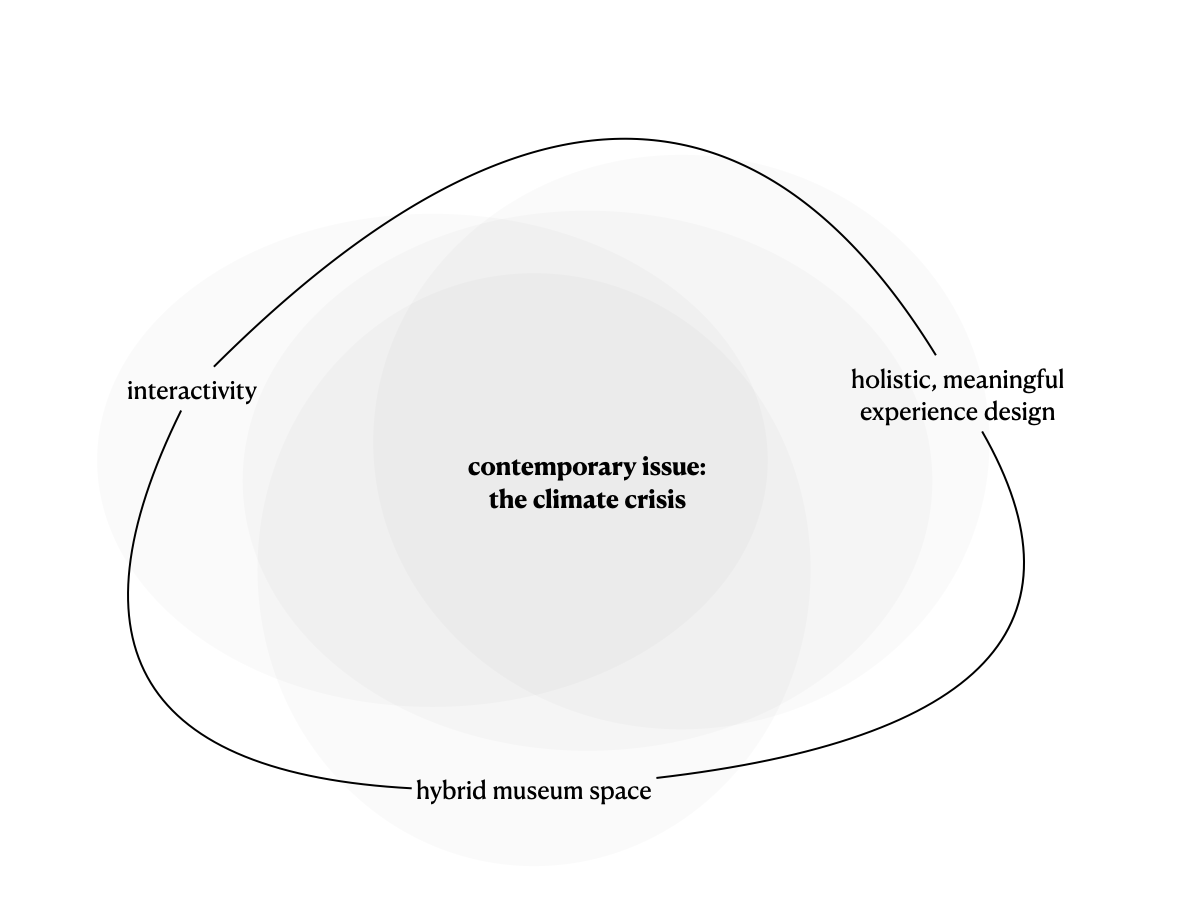
\includegraphics[width=12.5cm]{pictures/Theory/problem_sphere.png}
\caption{My representation of sustainability issues in museums}
\end{figure}


\begin{figure}[H]
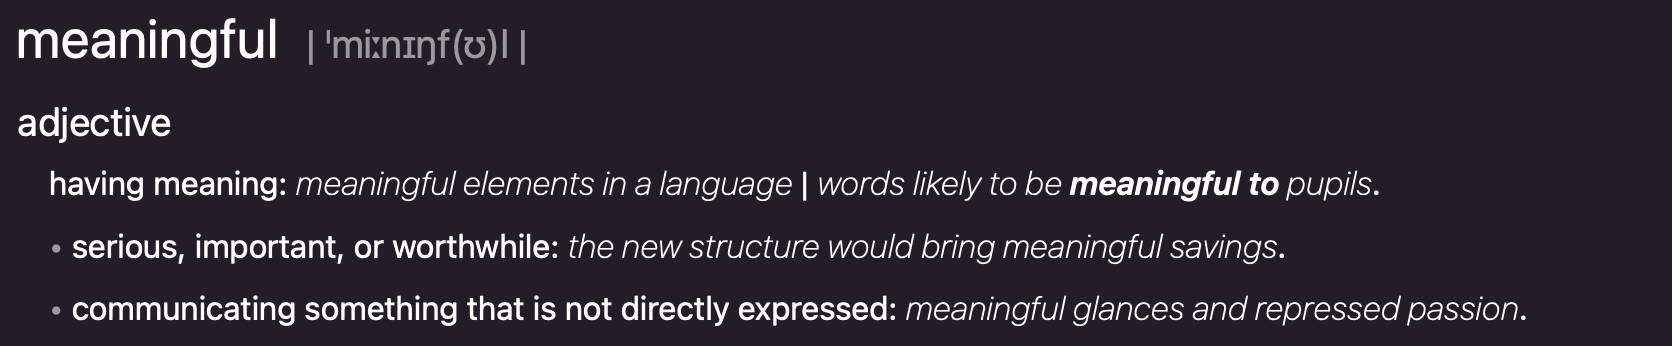
\includegraphics[width=12.5cm]{pictures/background/meaningful.png}
\caption{Meaningfulness}{\autocite{Oxford_dictionary}}
\centering
\end{figure}

The practical application of this analytical tool is something like this (the tables underneath), where I have plotted in the different installations and exhibitions to their respective tables. A thoruough walkthrough of the analysis is accounted for in Chapter 9: Analysis.
